\SourceLeaf{320}
Derselbe Satz ist übrigens auch umgekehrt wahr, die unverträglichen Data
werden verträglich, wenn man Eine der drei Richtungen in die entgegengesetzte
abändert, nur ist hier die abzuändernde nicht mehr willkürlich.

Wenn also z.\,B. unter den obigen vier Zeichnungen die erste (für ein
bestimmtes gegebenes Dreieck $ABC$) möglich ist, nemlich

\begin{center}\resizebox{6.8cm}{!}{%
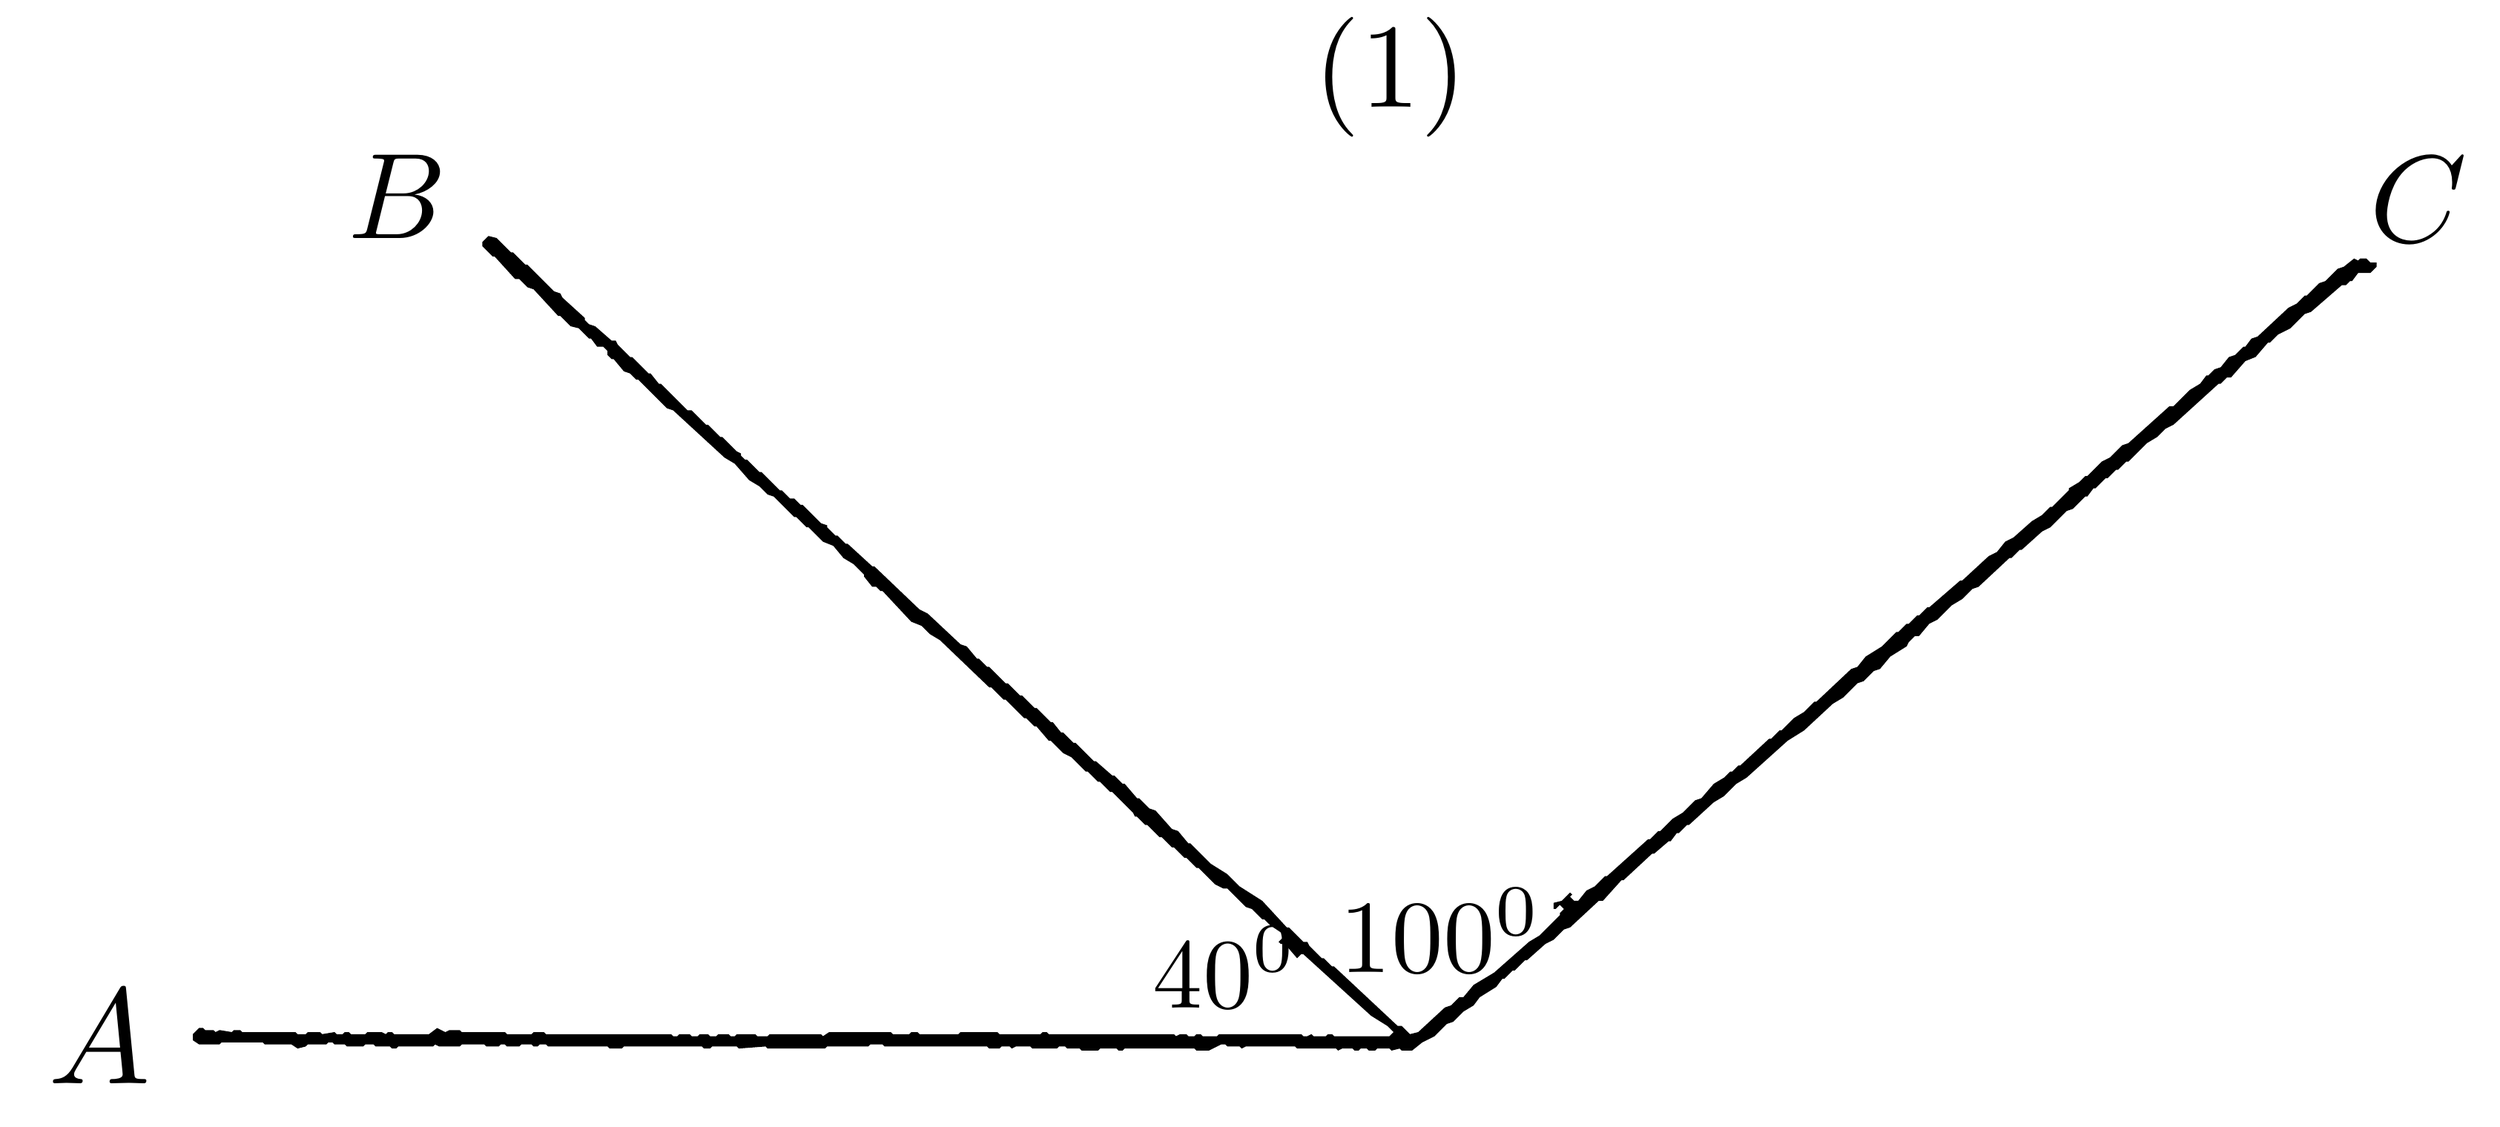
\begin{tikzpicture}[x=1pt,y=-1pt]
\path[use as bounding box] (0,0) rectangle (1198,529);
\path[fill=black,draw=none,even odd rule]
(84,497) -- (87,499) -- (97,499) -- (98,498) -- (118,498) -- (119,499) -- (132,499) -- (135,501) -- (139,500) -- (140,499) -- (149,499) -- (150,498) -- (152,498) -- (153,499) -- (158,499) -- (159,500) -- (167,500) -- (168,499) -- (172,499) -- (173,500) -- (180,500) -- (181,501) -- (183,501) -- (184,500) -- (201,500) -- (202,499) -- (204,500) -- (214,500) -- (215,499) -- (226,499) -- (227,500) -- (233,500) -- (234,499) -- (236,499) -- (237,500) -- (243,500) -- (244,499) -- (249,499) -- (250,500) -- (252,500) -- (253,499) -- (256,499) -- (257,500) -- (286,500) -- (287,501) -- (293,501) -- (294,500) -- (332,500) -- (333,501) -- (336,501) -- (337,500) -- (349,500) -- (350,501) -- (363,500) -- (364,501) -- (392,501) -- (393,500) -- (413,500) -- (414,499) -- (420,499) -- (421,500) -- (471,500) -- (472,501) -- (477,501) -- (478,500) -- (482,500) -- (483,501) -- (485,500) -- (492,500) -- (493,501) -- (505,501) -- (506,500) -- (509,500) -- (510,501) -- (516,501) -- (517,502) -- (525,502) -- (526,501) -- (534,501) -- (535,502) -- (537,502) -- (538,501) -- (572,501) -- (573,502) -- (579,502) -- (585,499) -- (587,499) -- (588,500) -- (594,500) -- (595,501) -- (597,500) -- (621,500) -- (622,501) -- (641,501) -- (642,502) -- (644,501) -- (649,501) -- (650,502) -- (652,502) -- (653,501) -- (656,501) -- (657,502) -- (660,502) -- (661,501) -- (667,501) -- (668,502) -- (672,501) -- (673,502) -- (678,502) -- (683,498) -- (689,495) -- (695,489) -- (698,488) -- (703,483) -- (708,480) -- (711,476) -- (719,471) -- (722,467) -- (723,467) -- (727,463) -- (728,463) -- (733,458) -- (734,458) -- (743,450) -- (747,448) -- (752,443) -- (755,442) -- (769,429) -- (771,429) -- (780,419) -- (781,419) -- (795,406) -- (796,406) -- (803,400) -- (804,400) -- (807,396) -- (808,396) -- (812,392) -- (813,392) -- (825,381) -- (830,378) -- (836,372) -- (841,369) -- (861,351) -- (869,346) -- (883,333) -- (888,330) -- (895,323) -- (898,322) -- (903,317) -- (906,316) -- (911,310) -- (919,305) -- (920,303) -- (923,300) -- (925,300) -- (930,294) -- (934,292) -- (941,285) -- (946,282) -- (951,277) -- (954,276) -- (969,262) -- (970,262) -- (974,258) -- (975,258) -- (985,249) -- (989,247) -- (997,239) -- (1000,238) -- (1006,232) -- (1007,232) -- (1010,228) -- (1011,228) -- (1016,223) -- (1017,223) -- (1021,219) -- (1022,219) -- (1026,215) -- (1027,215) -- (1036,206) -- (1041,203) -- (1045,199) -- (1049,197) -- (1071,177) -- (1072,177) -- (1075,174) -- (1077,174) -- (1084,166) -- (1089,164) -- (1095,157) -- (1096,157) -- (1100,153) -- (1106,150) -- (1113,143) -- (1116,142) -- (1131,129) -- (1133,129) -- (1135,127) -- (1136,127) -- (1139,123) -- (1145,123) -- (1148,120) -- (1148,118) -- (1145,118) -- (1143,116) -- (1140,116) -- (1139,117) -- (1137,116) -- (1132,120) -- (1129,121) -- (1123,127) -- (1120,128) -- (1114,134) -- (1113,134) -- (1109,138) -- (1105,140) -- (1090,154) -- (1087,155) -- (1084,159) -- (1083,159) -- (1079,163) -- (1076,164) -- (1072,169) -- (1069,170) -- (1066,173) -- (1065,173) -- (1062,177) -- (1057,180) -- (1049,188) -- (1047,188) -- (1027,206) -- (1024,207) -- (1018,213) -- (1014,215) -- (1007,222) -- (1006,222) -- (1003,225) -- (998,228) -- (998,229) -- (990,237) -- (989,237) -- (985,241) -- (980,244) -- (971,252) -- (967,254) -- (963,259) -- (959,261) -- (946,273) -- (945,273) -- (930,286) -- (929,286) -- (925,290) -- (924,290) -- (920,294) -- (919,294) -- (915,298) -- (914,298) -- (907,305) -- (899,310) -- (895,315) -- (892,316) -- (875,332) -- (874,332) -- (869,337) -- (864,340) -- (858,346) -- (857,346) -- (853,350) -- (852,350) -- (838,363) -- (837,363) -- (834,366) -- (833,366) -- (830,369) -- (825,372) -- (819,379) -- (816,380) -- (810,386) -- (805,389) -- (799,395) -- (798,395) -- (794,399) -- (793,399) -- (773,417) -- (772,417) -- (767,422) -- (763,424) -- (759,429) -- (757,429) -- (755,427) -- (756,426) -- (755,425) -- (751,429) -- (747,430) -- (747,433) -- (748,433) -- (750,431) -- (752,433) -- (750,435) -- (750,436) -- (740,446) -- (735,449) -- (718,464) -- (708,470) -- (703,476) -- (701,476) -- (697,480) -- (694,481) -- (681,493) -- (677,494) -- (673,490) -- (671,490) -- (640,461) -- (639,461) -- (635,457) -- (634,457) -- (628,451) -- (627,449) -- (625,449) -- (618,442) -- (617,442) -- (605,429) -- (594,422) -- (588,416) -- (580,411) -- (570,401) -- (569,401) -- (564,395) -- (561,394) -- (553,385) -- (550,384) -- (545,379) -- (544,379) -- (538,372) -- (537,372) -- (533,368) -- (532,368) -- (524,361) -- (523,361) -- (514,352) -- (513,352) -- (508,347) -- (507,347) -- (503,342) -- (502,342) -- (495,335) -- (494,335) -- (488,329) -- (487,329) -- (481,323) -- (480,323) -- (472,315) -- (471,315) -- (467,311) -- (466,311) -- (461,305) -- (458,304) -- (442,289) -- (438,287) -- (416,266) -- (415,266) -- (403,255) -- (402,255) -- (398,251) -- (397,251) -- (393,247) -- (393,246) -- (390,245) -- (381,236) -- (380,236) -- (377,233) -- (375,233) -- (371,229) -- (370,229) -- (361,220) -- (360,220) -- (354,214) -- (353,214) -- (351,212) -- (351,211) -- (349,210) -- (342,203) -- (341,203) -- (335,197) -- (334,197) -- (327,190) -- (325,190) -- (312,177) -- (311,177) -- (307,172) -- (306,172) -- (298,164) -- (297,164) -- (291,158) -- (290,156) -- (288,156) -- (280,149) -- (277,148) -- (275,146) -- (275,145) -- (264,135) -- (263,133) -- (260,132) -- (247,119) -- (246,119) -- (240,113) -- (239,113) -- (232,106) -- (228,105) -- (225,108) -- (225,110) -- (230,115) -- (231,115) -- (241,126) -- (243,126) -- (247,130) -- (250,131) -- (262,144) -- (263,144) -- (268,149) -- (272,150) -- (277,155) -- (278,155) -- (281,159) -- (284,159) -- (286,161) -- (286,163) -- (288,165) -- (289,165) -- (294,171) -- (297,172) -- (300,175) -- (301,175) -- (315,189) -- (318,190) -- (343,213) -- (348,216) -- (355,224) -- (360,227) -- (364,231) -- (367,232) -- (377,242) -- (378,242) -- (383,247) -- (384,247) -- (391,254) -- (396,256) -- (401,262) -- (406,265) -- (411,270) -- (411,271) -- (415,276) -- (417,276) -- (419,278) -- (420,278) -- (434,293) -- (439,295) -- (443,299) -- (448,302) -- (472,325) -- (473,325) -- (479,331) -- (480,331) -- (489,340) -- (490,340) -- (494,344) -- (495,344) -- (501,351) -- (502,351) -- (508,357) -- (512,359) -- (519,366) -- (520,366) -- (525,371) -- (526,371) -- (531,376) -- (532,376) -- (542,386) -- (543,388) -- (544,388) -- (548,392) -- (549,392) -- (555,398) -- (556,398) -- (561,403) -- (562,403) -- (567,408) -- (568,408) -- (573,413) -- (574,413) -- (582,421) -- (586,423) -- (588,423) -- (597,432) -- (600,433) -- (605,438) -- (606,438) -- (609,441) -- (615,445) -- (615,447) -- (613,449) -- (614,450) -- (616,450) -- (622,457) -- (624,455) -- (625,455) -- (658,485) -- (666,490) -- (669,493) -- (667,495) -- (640,495) -- (639,494) -- (637,494) -- (636,495) -- (630,495) -- (629,494) -- (627,495) -- (625,495) -- (624,494) -- (584,494) -- (583,495) -- (576,495) -- (575,494) -- (573,494) -- (572,495) -- (569,495) -- (568,494) -- (565,494) -- (563,495) -- (562,494) -- (501,494) -- (500,493) -- (498,493) -- (497,494) -- (477,494) -- (476,493) -- (458,493) -- (457,494) -- (438,494) -- (437,493) -- (434,493) -- (433,494) -- (425,494) -- (424,493) -- (394,493) -- (391,495) -- (390,494) -- (365,494) -- (364,495) -- (359,495) -- (358,494) -- (349,494) -- (348,495) -- (346,495) -- (345,494) -- (340,494) -- (339,495) -- (336,495) -- (335,494) -- (331,494) -- (330,495) -- (327,495) -- (326,494) -- (321,494) -- (320,495) -- (318,495) -- (317,494) -- (256,494) -- (255,493) -- (250,493) -- (249,494) -- (237,494) -- (236,493) -- (215,493) -- (214,492) -- (209,492) -- (207,493) -- (203,491) -- (199,494) -- (182,494) -- (181,493) -- (179,493) -- (178,494) -- (176,493) -- (169,493) -- (168,494) -- (161,494) -- (160,493) -- (158,493) -- (157,494) -- (154,494) -- (153,493) -- (147,494) -- (146,493) -- (140,493) -- (139,494) -- (135,494) -- (134,493) -- (108,493) -- (107,492) -- (104,492) -- (103,493) -- (97,492) -- (95,493) -- (94,492) -- (90,492) -- (89,491) -- (87,491) -- (84,494) -- cycle;
\node[inner sep=0pt,font=\fontsize{10}{10}\selectfont] at (667.5,27.5) {\scalebox{5.841}{$(1)$}};
\node[inner sep=0pt,font=\fontsize{10}{10}\selectfont] at (183.5,86.0) {\scalebox{5.94}{$B$}};
\node[inner sep=0pt,font=\fontsize{10}{10}\selectfont] at (1168.5,87.5) {\scalebox{6.039}{$C$}};
\node[inner sep=0pt,font=\fontsize{10}{10}\selectfont] at (38.5,495.5) {\scalebox{6.633}{$A$}};
\node[inner sep=0pt,font=\fontsize{10}{10}\selectfont] at (587.0,461.5) {\scalebox{4.851}{$40^0$}};
\node[inner sep=0pt,font=\fontsize{10}{10}\selectfont] at (692.0,443.5) {\scalebox{5.049}{$100^0$}};
\end{tikzpicture}%
}
\end{center}

möglich, so sind

\begin{center}\resizebox{3.1cm}{!}{%
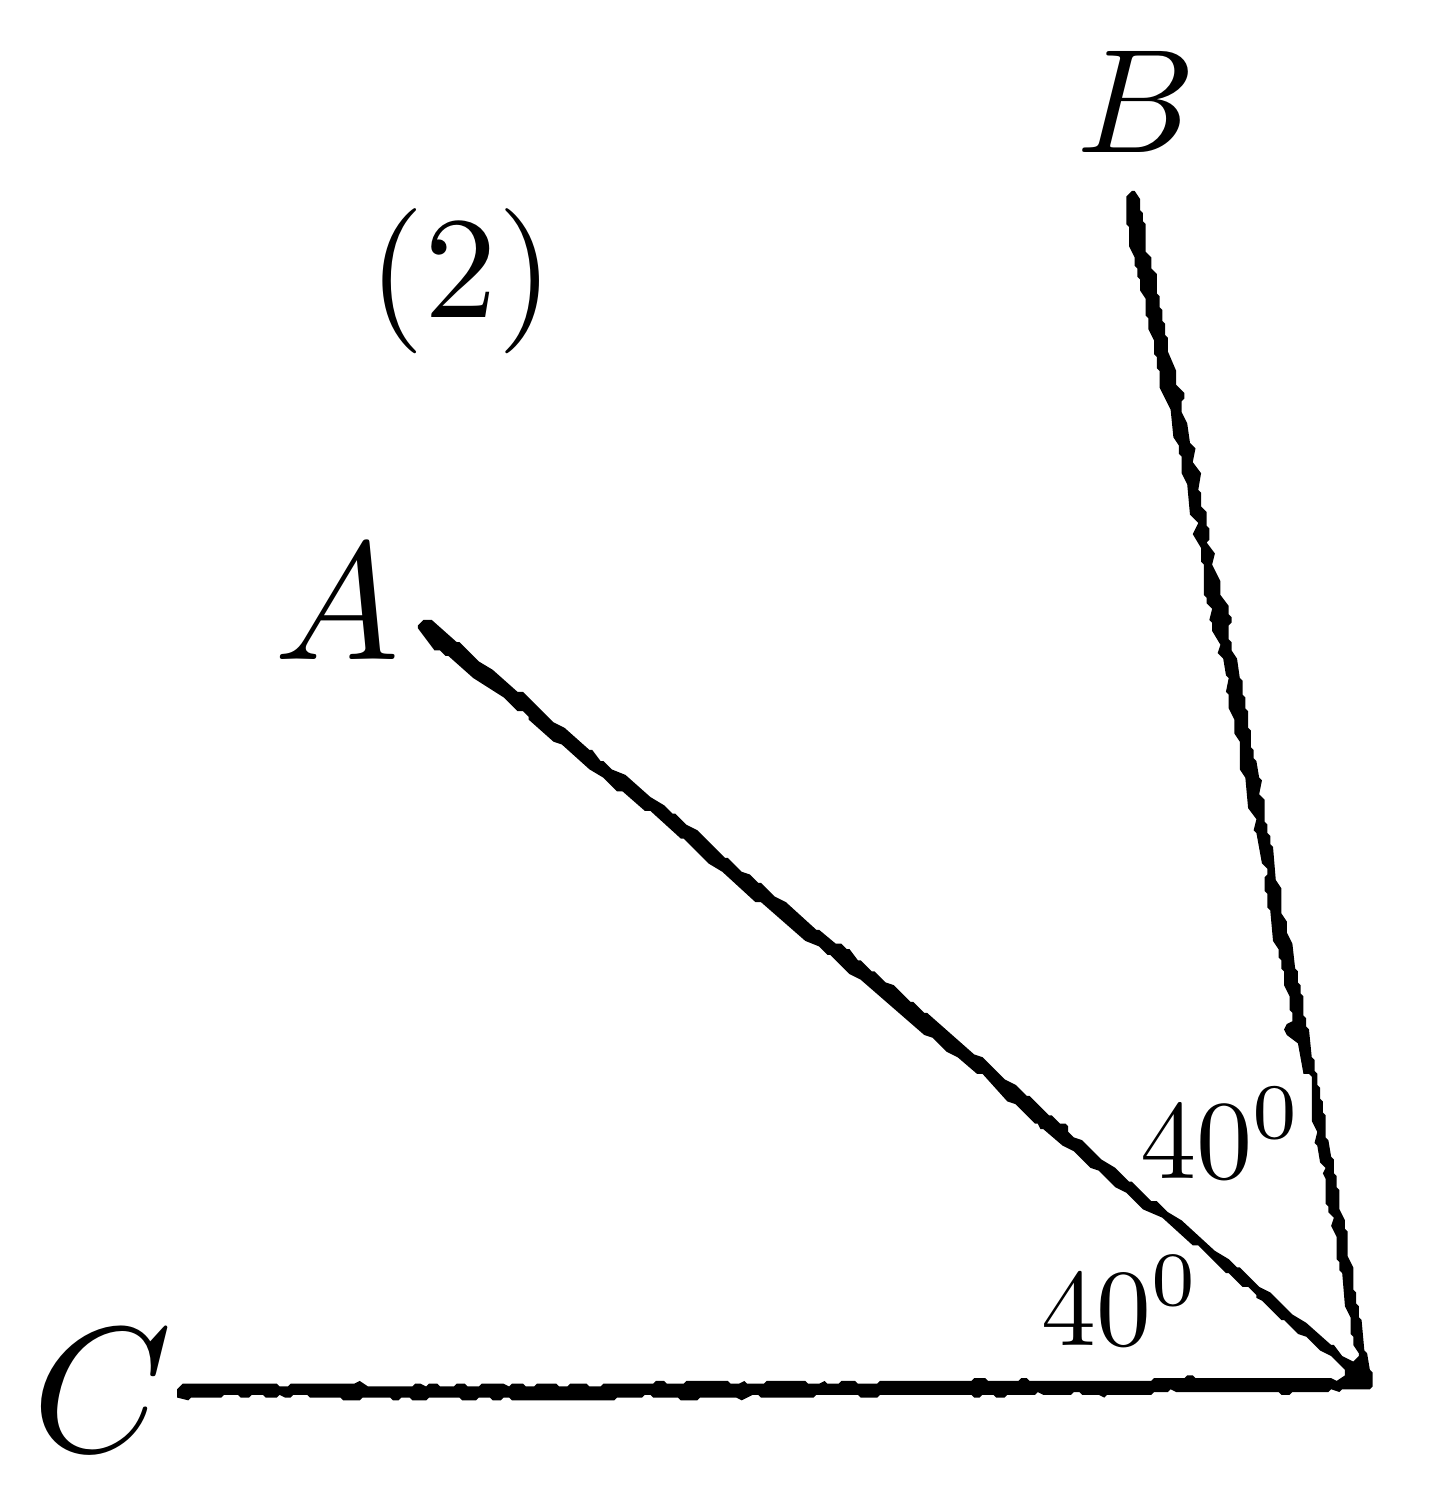
\begin{tikzpicture}[x=1pt,y=-1pt]
\path[use as bounding box] (0,0) rectangle (497,525);
\path[fill=black,draw=none,even odd rule]
(400,59) -- (399,59) -- (397,61) -- (397,71) -- (398,72) -- (398,79) -- (400,83) -- (400,86) -- (401,87) -- (401,90) -- (402,91) -- (402,95) -- (404,98) -- (404,104) -- (405,105) -- (405,109) -- (407,113) -- (407,118) -- (408,119) -- (408,123) -- (409,124) -- (409,130) -- (413,138) -- (414,148) -- (416,151) -- (416,154) -- (417,155) -- (417,161) -- (419,165) -- (420,176) -- (423,179) -- (421,183) -- (424,188) -- (424,193) -- (425,194) -- (425,205) -- (426,206) -- (426,208) -- (428,210) -- (427,214) -- (428,215) -- (428,218) -- (431,223) -- (430,226) -- (432,228) -- (433,234) -- (434,235) -- (433,240) -- (434,241) -- (434,246) -- (436,250) -- (436,255) -- (438,258) -- (438,268) -- (440,271) -- (441,282) -- (444,286) -- (443,290) -- (444,291) -- (446,302) -- (448,304) -- (448,306) -- (447,307) -- (447,312) -- (448,313) -- (448,318) -- (449,319) -- (450,330) -- (452,333) -- (452,336) -- (453,337) -- (453,340) -- (454,341) -- (454,346) -- (456,350) -- (456,355) -- (457,356) -- (457,359) -- (455,360) -- (454,362) -- (455,364) -- (459,367) -- (461,378) -- (463,378) -- (464,379) -- (464,395) -- (466,399) -- (465,403) -- (466,404) -- (467,410) -- (469,412) -- (468,414) -- (469,416) -- (469,425) -- (470,426) -- (470,428) -- (472,430) -- (471,433) -- (473,437) -- (473,445) -- (474,446) -- (474,449) -- (475,450) -- (476,462) -- (478,466) -- (478,472) -- (479,473) -- (479,476) -- (481,479) -- (481,480) -- (479,482) -- (475,480) -- (472,476) -- (471,476) -- (462,468) -- (457,465) -- (449,457) -- (445,455) -- (438,448) -- (437,448) -- (434,445) -- (429,442) -- (417,431) -- (412,428) -- (408,424) -- (406,424) -- (399,417) -- (398,417) -- (393,412) -- (388,409) -- (381,402) -- (378,401) -- (376,399) -- (376,397) -- (375,396) -- (373,396) -- (370,393) -- (369,393) -- (362,386) -- (361,386) -- (357,382) -- (353,380) -- (345,372) -- (342,371) -- (325,356) -- (324,356) -- (320,352) -- (319,352) -- (313,346) -- (310,345) -- (306,341) -- (305,341) -- (301,337) -- (300,337) -- (297,333) -- (296,333) -- (294,331) -- (292,331) -- (286,326) -- (285,326) -- (274,316) -- (270,314) -- (265,309) -- (264,309) -- (261,306) -- (258,305) -- (253,300) -- (252,300) -- (242,290) -- (238,288) -- (234,284) -- (233,284) -- (230,281) -- (225,278) -- (216,270) -- (211,268) -- (208,265) -- (207,265) -- (204,261) -- (203,261) -- (194,253) -- (190,251) -- (179,240) -- (177,240) -- (168,232) -- (163,229) -- (156,222) -- (155,222) -- (146,214) -- (143,214) -- (141,216) -- (141,217) -- (147,225) -- (149,225) -- (151,227) -- (152,227) -- (161,235) -- (172,242) -- (177,247) -- (179,247) -- (181,249) -- (181,250) -- (190,258) -- (193,259) -- (203,268) -- (208,271) -- (213,276) -- (215,276) -- (223,283) -- (225,283) -- (236,293) -- (237,293) -- (246,302) -- (251,305) -- (263,316) -- (265,316) -- (281,330) -- (286,332) -- (289,335) -- (290,335) -- (297,342) -- (301,344) -- (324,364) -- (327,365) -- (332,370) -- (336,372) -- (343,378) -- (345,378) -- (354,388) -- (357,389) -- (364,396) -- (365,396) -- (366,398) -- (367,398) -- (374,404) -- (378,406) -- (384,412) -- (387,413) -- (393,419) -- (397,421) -- (403,427) -- (410,430) -- (421,440) -- (423,440) -- (433,450) -- (434,450) -- (439,455) -- (441,455) -- (444,458) -- (444,459) -- (446,460) -- (453,467) -- (454,467) -- (459,472) -- (462,473) -- (467,478) -- (471,480) -- (476,485) -- (476,487) -- (473,489) -- (471,488) -- (422,488) -- (421,487) -- (419,487) -- (418,488) -- (407,488) -- (406,489) -- (362,489) -- (361,488) -- (359,488) -- (358,489) -- (347,489) -- (346,488) -- (342,488) -- (341,489) -- (308,489) -- (307,490) -- (300,490) -- (299,489) -- (294,489) -- (293,490) -- (289,490) -- (288,489) -- (286,490) -- (282,490) -- (281,489) -- (267,489) -- (266,490) -- (260,490) -- (259,489) -- (257,490) -- (254,490) -- (253,489) -- (238,489) -- (237,490) -- (231,490) -- (230,489) -- (227,489) -- (226,490) -- (208,490) -- (207,491) -- (203,491) -- (202,490) -- (196,490) -- (195,491) -- (192,491) -- (191,490) -- (184,490) -- (183,491) -- (180,491) -- (179,490) -- (175,490) -- (174,491) -- (172,490) -- (164,490) -- (163,491) -- (159,491) -- (158,490) -- (155,490) -- (154,491) -- (149,491) -- (148,490) -- (145,490) -- (144,491) -- (142,490) -- (140,490) -- (139,491) -- (123,491) -- (120,489) -- (118,490) -- (95,490) -- (94,491) -- (91,491) -- (90,490) -- (56,490) -- (54,492) -- (54,495) -- (58,496) -- (59,495) -- (70,495) -- (71,494) -- (76,494) -- (77,495) -- (80,495) -- (81,494) -- (85,494) -- (86,495) -- (90,495) -- (91,494) -- (93,495) -- (95,495) -- (96,494) -- (101,494) -- (102,495) -- (113,495) -- (114,496) -- (120,496) -- (121,495) -- (131,495) -- (132,496) -- (134,496) -- (135,495) -- (138,495) -- (139,496) -- (144,496) -- (145,495) -- (156,495) -- (157,496) -- (162,496) -- (163,495) -- (167,495) -- (168,496) -- (171,496) -- (172,495) -- (174,495) -- (175,496) -- (212,496) -- (213,495) -- (222,495) -- (223,494) -- (225,494) -- (226,495) -- (235,495) -- (236,496) -- (242,496) -- (243,495) -- (256,495) -- (258,496) -- (262,494) -- (264,494) -- (265,495) -- (284,495) -- (285,494) -- (300,494) -- (301,495) -- (307,495) -- (308,494) -- (341,494) -- (342,495) -- (344,495) -- (345,494) -- (349,494) -- (350,495) -- (353,495) -- (354,494) -- (364,494) -- (365,493) -- (367,494) -- (377,494) -- (378,493) -- (380,493) -- (381,494) -- (387,494) -- (389,495) -- (390,494) -- (406,494) -- (407,493) -- (412,493) -- (413,492) -- (415,493) -- (452,493) -- (453,494) -- (456,494) -- (457,493) -- (470,493) -- (471,492) -- (474,493) -- (475,492) -- (485,492) -- (486,491) -- (486,486) -- (485,485) -- (484,479) -- (483,478) -- (482,467) -- (481,466) -- (481,462) -- (480,461) -- (480,457) -- (479,456) -- (479,448) -- (477,444) -- (477,435) -- (476,434) -- (476,431) -- (474,427) -- (474,420) -- (473,419) -- (473,415) -- (472,414) -- (472,409) -- (471,408) -- (470,402) -- (469,401) -- (469,393) -- (468,392) -- (468,388) -- (467,387) -- (467,383) -- (466,382) -- (466,378) -- (465,377) -- (465,373) -- (464,372) -- (463,362) -- (462,361) -- (462,358) -- (461,357) -- (461,350) -- (460,349) -- (460,346) -- (459,345) -- (459,341) -- (458,340) -- (457,331) -- (455,327) -- (455,323) -- (453,320) -- (453,311) -- (451,308) -- (450,296) -- (449,295) -- (449,292) -- (448,291) -- (448,288) -- (447,287) -- (447,279) -- (445,277) -- (446,272) -- (445,271) -- (444,265) -- (443,264) -- (443,261) -- (442,260) -- (442,254) -- (441,253) -- (441,247) -- (440,246) -- (440,242) -- (439,241) -- (439,236) -- (438,235) -- (437,228) -- (435,225) -- (435,222) -- (434,221) -- (434,216) -- (435,215) -- (435,213) -- (434,212) -- (434,209) -- (431,205) -- (431,200) -- (428,194) -- (429,190) -- (426,186) -- (427,185) -- (427,181) -- (426,180) -- (426,175) -- (424,173) -- (424,168) -- (423,167) -- (424,161) -- (421,157) -- (422,152) -- (420,150) -- (419,143) -- (417,139) -- (417,135) -- (418,134) -- (418,132) -- (415,129) -- (415,124) -- (412,117) -- (412,112) -- (411,111) -- (411,107) -- (410,106) -- (410,102) -- (409,101) -- (409,97) -- (408,96) -- (408,89) -- (406,87) -- (406,83) -- (404,81) -- (404,71) -- (403,70) -- (403,67) -- (402,66) -- (402,62) -- cycle;
\node[inner sep=0pt,font=\fontsize{10}{10}\selectfont] at (156.5,91.5) {\scalebox{5.247}{$(2)$}};
\node[inner sep=0pt,font=\fontsize{10}{10}\selectfont] at (400.5,27.0) {\scalebox{5.346}{$B$}};
\node[inner sep=0pt,font=\fontsize{10}{10}\selectfont] at (112.0,207.5) {\scalebox{6.039}{$A$}};
\node[inner sep=0pt,font=\fontsize{10}{10}\selectfont] at (27.0,492.5) {\scalebox{6.435}{$C$}};
\node[inner sep=0pt,font=\fontsize{10}{10}\selectfont] at (431.5,399.5) {\scalebox{4.059}{$40^0$}};
\node[inner sep=0pt,font=\fontsize{10}{10}\selectfont] at (395.0,460.0) {\scalebox{3.96}{$40^0$}};
\end{tikzpicture}%
}
\quad \resizebox{4.7cm}{!}{%
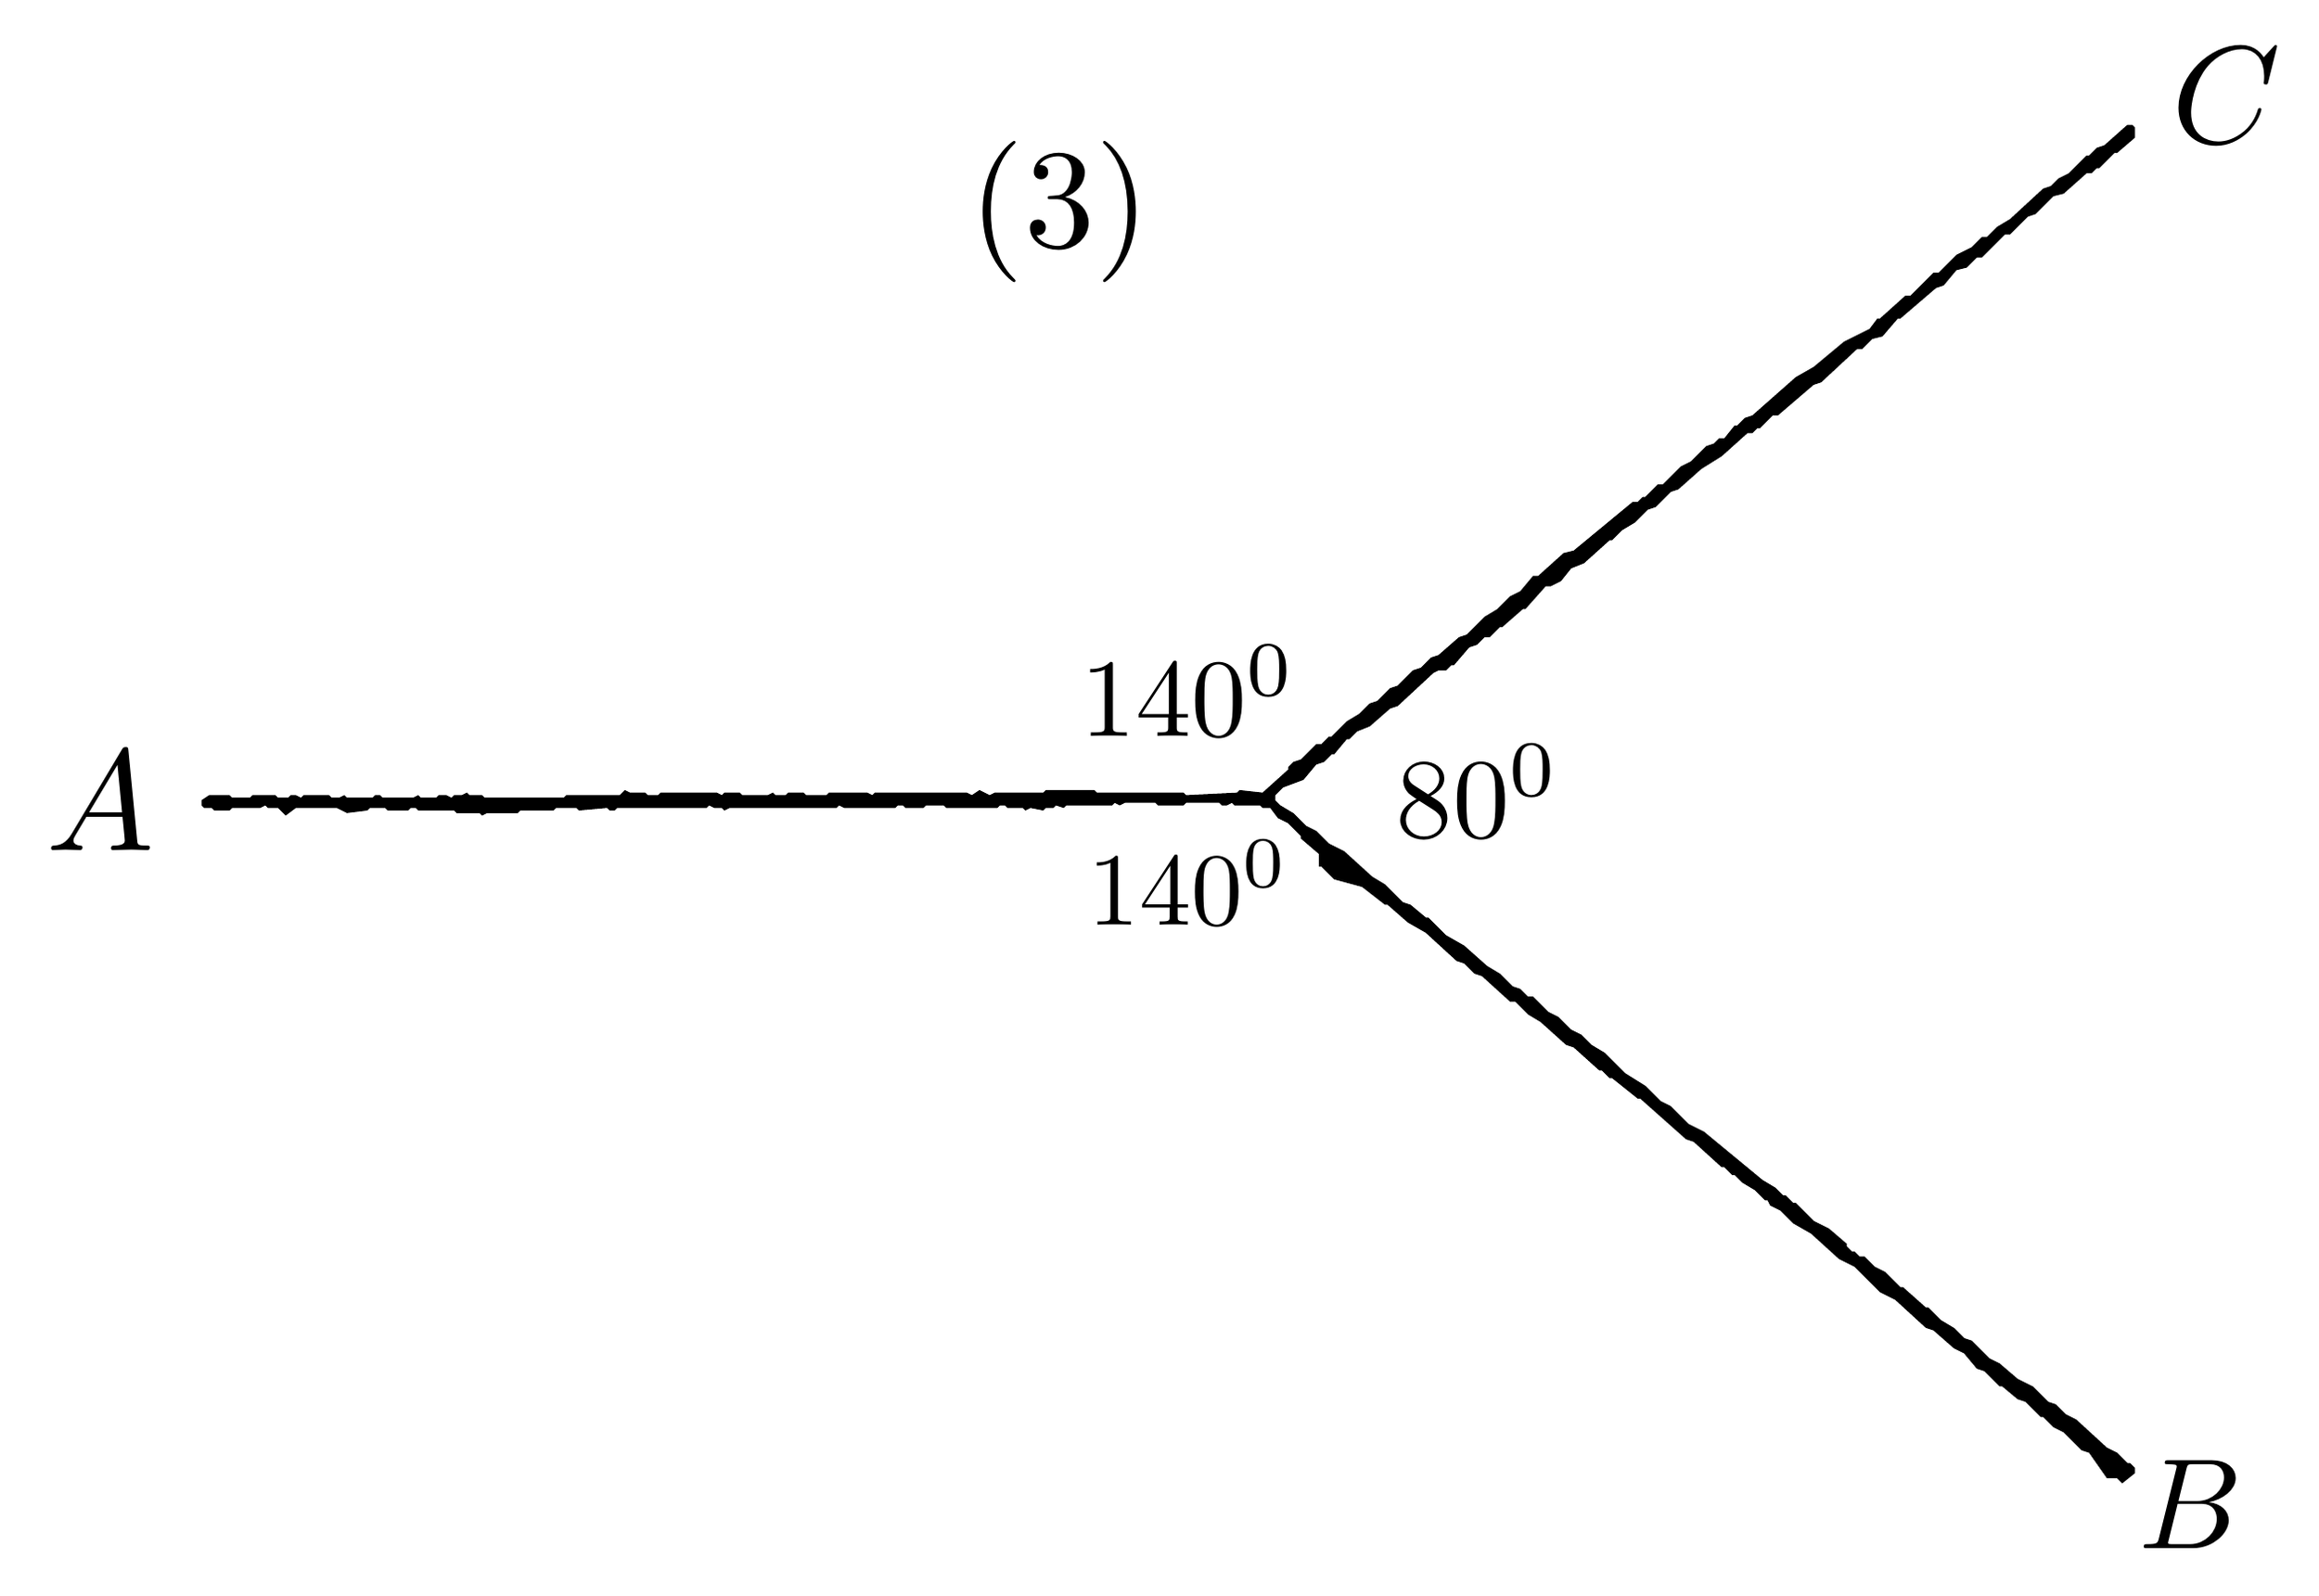
\begin{tikzpicture}[x=1pt,y=-1pt]
\path[use as bounding box] (0,0) rectangle (889,606);
\path[fill=black,draw=none,even odd rule]
(827,40) -- (826,39) -- (824,39) -- (815,47) -- (812,48) -- (809,51) -- (808,51) -- (801,58) -- (797,60) -- (794,63) -- (791,64) -- (778,76) -- (773,79) -- (769,83) -- (767,83) -- (763,87) -- (757,90) -- (750,97) -- (748,97) -- (739,106) -- (737,106) -- (727,115) -- (726,115) -- (723,119) -- (713,124) -- (701,134) -- (694,138) -- (677,153) -- (674,154) -- (671,157) -- (670,157) -- (666,162) -- (664,162) -- (662,164) -- (659,165) -- (653,171) -- (649,173) -- (642,180) -- (640,180) -- (635,185) -- (634,185) -- (632,187) -- (630,187) -- (607,206) -- (603,207) -- (593,216) -- (591,216) -- (586,222) -- (582,224) -- (577,229) -- (572,232) -- (565,239) -- (562,240) -- (554,247) -- (551,248) -- (547,252) -- (544,253) -- (538,259) -- (535,260) -- (530,265) -- (527,266) -- (523,270) -- (518,273) -- (512,279) -- (511,279) -- (508,282) -- (506,282) -- (500,288) -- (497,289) -- (495,291) -- (495,292) -- (485,301) -- (476,300) -- (475,301) -- (455,302) -- (454,301) -- (420,301) -- (419,300) -- (400,300) -- (399,301) -- (380,301) -- (378,302) -- (374,300) -- (371,302) -- (369,301) -- (333,301) -- (332,302) -- (330,301) -- (315,301) -- (314,302) -- (306,302) -- (305,301) -- (299,301) -- (298,302) -- (294,302) -- (293,301) -- (291,302) -- (281,302) -- (280,301) -- (274,301) -- (273,302) -- (271,301) -- (249,301) -- (248,302) -- (244,302) -- (243,301) -- (237,301) -- (235,300) -- (233,302) -- (212,302) -- (211,303) -- (180,303) -- (179,302) -- (174,302) -- (173,301) -- (171,302) -- (168,302) -- (167,303) -- (165,302) -- (162,302) -- (161,303) -- (155,303) -- (154,302) -- (152,303) -- (140,303) -- (139,302) -- (137,302) -- (136,303) -- (126,303) -- (125,302) -- (123,303) -- (120,303) -- (119,302) -- (109,302) -- (108,303) -- (106,302) -- (104,302) -- (103,303) -- (99,303) -- (98,302) -- (89,302) -- (88,303) -- (81,303) -- (80,302) -- (72,302) -- (69,304) -- (69,306) -- (70,307) -- (73,307) -- (74,308) -- (80,308) -- (81,307) -- (92,307) -- (94,306) -- (95,307) -- (99,307) -- (102,310) -- (106,307) -- (122,307) -- (126,309) -- (134,308) -- (135,307) -- (141,307) -- (142,308) -- (150,308) -- (151,307) -- (153,307) -- (154,308) -- (168,308) -- (169,309) -- (178,309) -- (179,310) -- (181,309) -- (193,309) -- (194,308) -- (207,308) -- (208,307) -- (216,307) -- (217,308) -- (228,307) -- (229,308) -- (231,308) -- (232,307) -- (267,307) -- (268,306) -- (270,307) -- (273,307) -- (274,308) -- (276,307) -- (318,307) -- (319,306) -- (321,307) -- (341,307) -- (342,306) -- (344,306) -- (345,307) -- (352,307) -- (353,306) -- (360,306) -- (361,307) -- (381,307) -- (382,306) -- (384,306) -- (385,307) -- (391,307) -- (392,308) -- (394,307) -- (399,308) -- (400,307) -- (403,307) -- (404,306) -- (407,307) -- (408,306) -- (426,306) -- (427,305) -- (429,306) -- (431,305) -- (443,305) -- (444,306) -- (454,306) -- (455,305) -- (468,305) -- (469,306) -- (471,306) -- (473,305) -- (474,306) -- (484,306) -- (485,307) -- (488,307) -- (491,311) -- (495,313) -- (500,318) -- (500,319) -- (507,325) -- (507,330) -- (508,330) -- (513,335) -- (524,338) -- (533,345) -- (534,345) -- (542,352) -- (549,356) -- (561,367) -- (564,368) -- (568,372) -- (571,373) -- (582,383) -- (584,383) -- (589,388) -- (594,391) -- (604,400) -- (607,401) -- (617,410) -- (618,410) -- (621,413) -- (622,413) -- (632,421) -- (633,421) -- (651,437) -- (654,438) -- (665,448) -- (666,448) -- (669,451) -- (670,451) -- (673,454) -- (678,457) -- (682,461) -- (683,461) -- (684,463) -- (688,465) -- (693,470) -- (700,474) -- (711,484) -- (717,487) -- (727,497) -- (733,500) -- (745,511) -- (748,512) -- (756,519) -- (760,521) -- (765,527) -- (768,528) -- (774,534) -- (775,534) -- (781,539) -- (784,540) -- (790,546) -- (791,546) -- (795,550) -- (799,552) -- (806,559) -- (809,560) -- (816,570) -- (820,570) -- (822,572) -- (827,568) -- (827,566) -- (825,564) -- (824,564) -- (820,560) -- (816,558) -- (804,547) -- (800,545) -- (796,541) -- (793,540) -- (787,534) -- (781,531) -- (774,525) -- (770,523) -- (763,516) -- (760,515) -- (756,511) -- (751,508) -- (746,503) -- (745,503) -- (736,495) -- (735,495) -- (729,489) -- (725,487) -- (721,483) -- (719,483) -- (717,481) -- (716,481) -- (714,479) -- (714,478) -- (707,472) -- (701,469) -- (694,462) -- (693,462) -- (690,459) -- (689,459) -- (686,456) -- (681,453) -- (658,434) -- (652,431) -- (645,424) -- (641,422) -- (635,416) -- (627,411) -- (619,403) -- (614,400) -- (610,396) -- (606,394) -- (601,389) -- (597,387) -- (591,381) -- (589,381) -- (586,378) -- (583,377) -- (578,372) -- (573,369) -- (564,361) -- (557,357) -- (550,350) -- (549,350) -- (543,345) -- (540,344) -- (533,337) -- (528,334) -- (517,324) -- (511,321) -- (506,316) -- (502,314) -- (497,309) -- (492,306) -- (490,304) -- (490,302) -- (493,299) -- (501,296) -- (506,290) -- (509,289) -- (512,286) -- (513,286) -- (518,280) -- (519,280) -- (522,277) -- (527,275) -- (535,268) -- (538,267) -- (552,254) -- (554,253) -- (557,253) -- (559,251) -- (560,251) -- (566,244) -- (569,243) -- (572,240) -- (574,240) -- (578,236) -- (579,236) -- (587,229) -- (588,229) -- (596,220) -- (598,220) -- (602,218) -- (606,213) -- (611,211) -- (621,202) -- (622,202) -- (626,198) -- (631,195) -- (636,190) -- (639,189) -- (645,183) -- (648,182) -- (657,174) -- (665,169) -- (675,160) -- (677,160) -- (679,158) -- (680,158) -- (685,153) -- (687,153) -- (701,141) -- (704,140) -- (718,127) -- (720,127) -- (724,123) -- (728,122) -- (734,115) -- (735,115) -- (749,103) -- (752,102) -- (757,96) -- (761,95) -- (765,91) -- (767,91) -- (776,82) -- (778,82) -- (785,75) -- (788,74) -- (795,67) -- (799,66) -- (808,58) -- (810,58) -- (812,56) -- (813,56) -- (819,50) -- (820,50) -- (827,44) -- cycle;
\node[inner sep=0pt,font=\fontsize{10}{10}\selectfont] at (405.5,73.0) {\scalebox{5.544}{$(3)$}};
\node[inner sep=0pt,font=\fontsize{10}{10}\selectfont] at (863.0,27.5) {\scalebox{5.445}{$C$}};
\node[inner sep=0pt,font=\fontsize{10}{10}\selectfont] at (29.5,304.5) {\scalebox{5.643}{$A$}};
\node[inner sep=0pt,font=\fontsize{10}{10}\selectfont] at (849.0,580.5) {\scalebox{5.049}{$B$}};
\node[inner sep=0pt,font=\fontsize{10}{10}\selectfont] at (456.0,261.0) {\scalebox{4.356}{$140^0$}};
\node[inner sep=0pt,font=\fontsize{10}{10}\selectfont] at (456.0,336.5) {\scalebox{4.059}{$140^0$}};
\node[inner sep=0pt,font=\fontsize{10}{10}\selectfont] at (569.5,300.5) {\scalebox{4.455}{$80^0$}};
\end{tikzpicture}%
}
\quad \resizebox{4.6cm}{!}{%
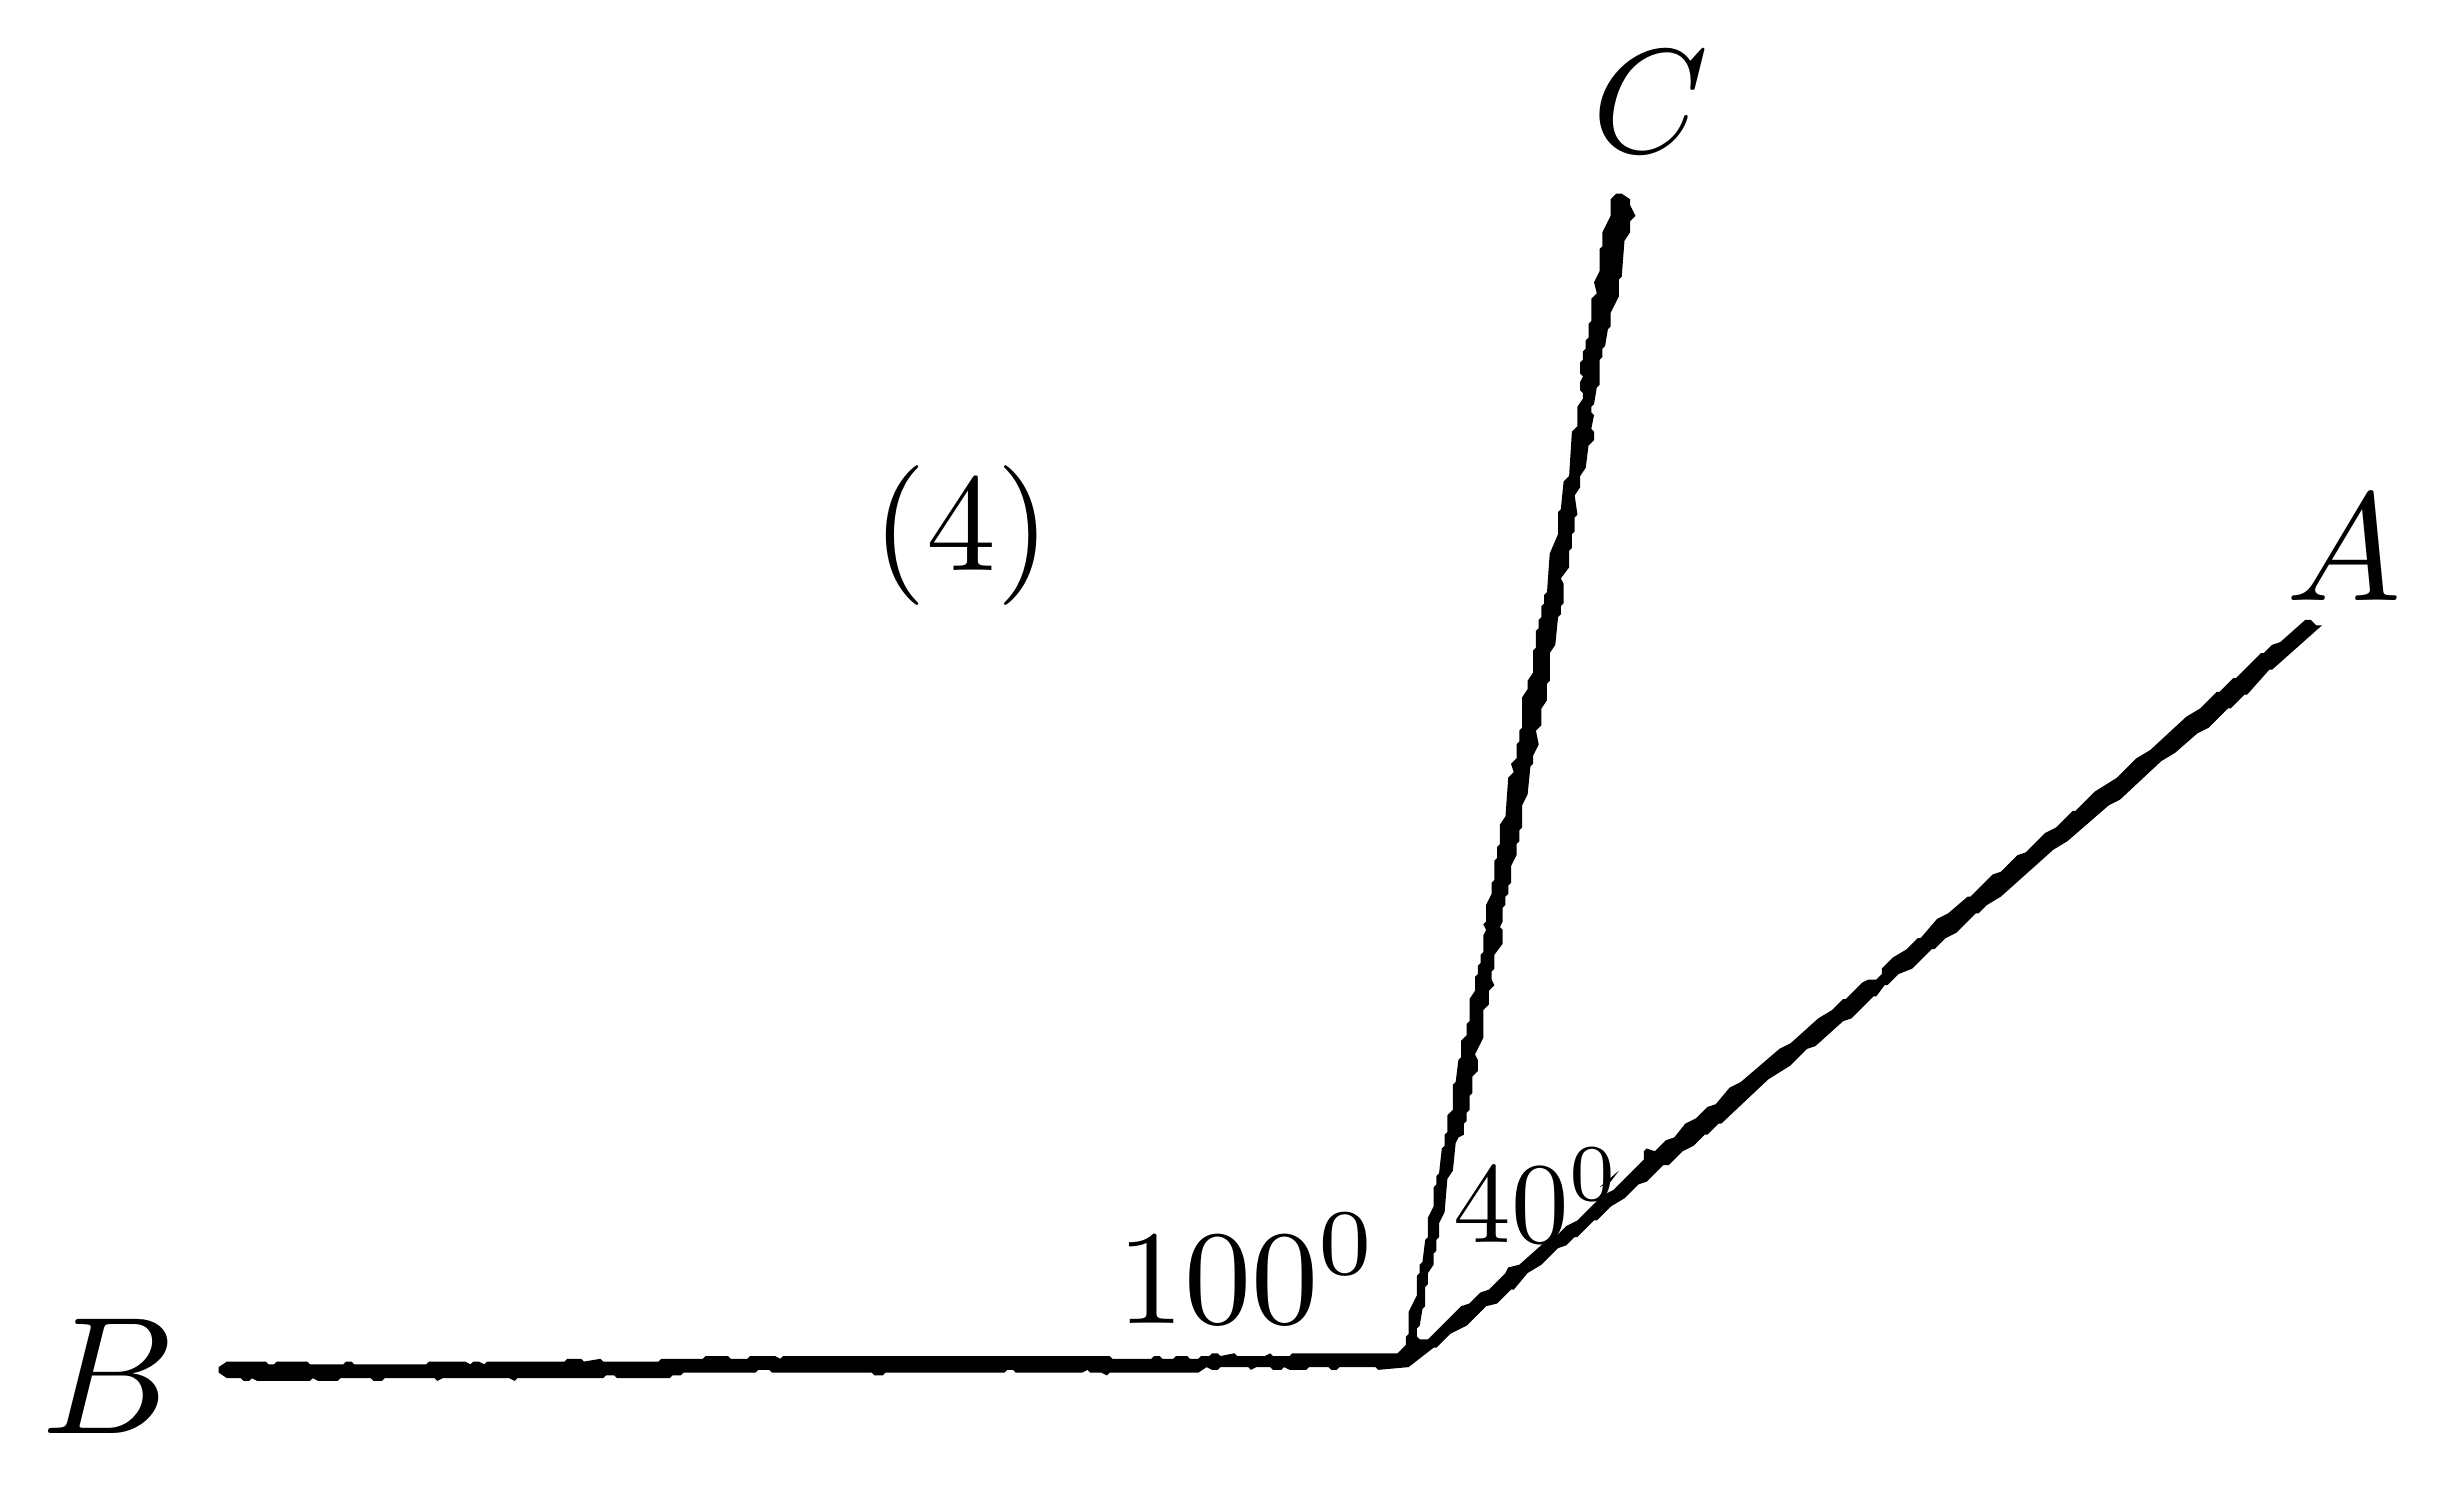
\begin{tikzpicture}[x=1pt,y=-1pt]
\path[use as bounding box] (0,0) rectangle (869,518);
\path[fill=black,draw=none,even odd rule]
(575,413) -- (568,419) -- (572,417) -- cycle
(829,216) -- (827,216) -- (825,214) -- (823,214) -- (814,222) -- (811,223) -- (808,226) -- (807,226) -- (798,235) -- (797,235) -- (792,240) -- (791,240) -- (785,246) -- (780,249) -- (767,261) -- (762,264) -- (755,271) -- (747,276) -- (740,283) -- (739,283) -- (733,289) -- (729,291) -- (722,298) -- (719,299) -- (713,305) -- (710,306) -- (702,314) -- (701,314) -- (694,320) -- (690,322) -- (684,329) -- (683,329) -- (679,333) -- (674,336) -- (670,340) -- (670,342) -- (668,344) -- (665,344) -- (663,345) -- (657,351) -- (656,351) -- (652,355) -- (647,358) -- (637,367) -- (633,369) -- (619,381) -- (615,383) -- (610,389) -- (607,390) -- (603,394) -- (599,396) -- (595,401) -- (592,402) -- (588,406) -- (585,405) -- (584,406) -- (584,409) -- (573,420) -- (569,422) -- (560,431) -- (556,433) -- (551,438) -- (548,439) -- (539,447) -- (535,448) -- (534,450) -- (528,456) -- (525,457) -- (521,461) -- (518,462) -- (506,474) -- (503,474) -- (502,473) -- (502,470) -- (503,469) -- (504,463) -- (505,462) -- (505,455) -- (506,454) -- (506,450) -- (508,447) -- (508,443) -- (509,442) -- (509,438) -- (510,437) -- (510,432) -- (512,428) -- (513,416) -- (515,413) -- (516,403) -- (517,401) -- (519,400) -- (519,396) -- (520,395) -- (520,392) -- (521,391) -- (521,386) -- (522,385) -- (522,379) -- (524,377) -- (524,373) -- (523,371) -- (526,365) -- (526,355) -- (528,353) -- (528,348) -- (530,346) -- (529,344) -- (529,341) -- (530,340) -- (530,335) -- (533,331) -- (533,326) -- (532,325) -- (533,323) -- (533,318) -- (534,317) -- (534,314) -- (535,313) -- (535,310) -- (536,309) -- (536,303) -- (538,299) -- (538,295) -- (539,294) -- (539,290) -- (540,289) -- (540,281) -- (542,277) -- (543,267) -- (544,266) -- (544,263) -- (546,259) -- (545,254) -- (547,252) -- (547,246) -- (549,243) -- (549,237) -- (550,236) -- (550,226) -- (552,223) -- (553,213) -- (554,212) -- (554,209) -- (555,208) -- (555,201) -- (554,199) -- (557,195) -- (557,189) -- (558,188) -- (558,183) -- (559,182) -- (559,177) -- (560,176) -- (559,169) -- (561,166) -- (561,162) -- (563,159) -- (564,151) -- (566,149) -- (566,146) -- (565,145) -- (566,140) -- (565,139) -- (565,137) -- (566,136) -- (567,130) -- (568,129) -- (568,120) -- (569,119) -- (569,116) -- (570,115) -- (571,109) -- (572,108) -- (572,103) -- (575,97) -- (575,91) -- (576,90) -- (577,77) -- (579,74) -- (579,70) -- (581,68) -- (579,64) -- (579,62) -- (576,60) -- (574,60) -- (572,62) -- (572,68) -- (569,74) -- (569,79) -- (568,80) -- (568,88) -- (566,92) -- (567,96) -- (565,98) -- (565,106) -- (564,107) -- (564,112) -- (563,113) -- (563,116) -- (562,117) -- (562,120) -- (561,121) -- (561,125) -- (562,126) -- (561,128) -- (561,131) -- (562,132) -- (562,134) -- (560,137) -- (560,144) -- (558,146) -- (557,162) -- (555,164) -- (554,174) -- (553,175) -- (553,183) -- (550,190) -- (549,204) -- (548,205) -- (548,208) -- (547,209) -- (547,213) -- (546,214) -- (546,217) -- (545,218) -- (545,224) -- (544,225) -- (544,233) -- (542,236) -- (542,239) -- (540,242) -- (540,253) -- (539,254) -- (539,258) -- (538,259) -- (538,264) -- (536,266) -- (537,269) -- (535,271) -- (534,285) -- (532,288) -- (532,295) -- (531,296) -- (531,300) -- (530,301) -- (530,308) -- (529,309) -- (529,313) -- (527,317) -- (527,323) -- (526,324) -- (527,326) -- (526,328) -- (526,334) -- (525,335) -- (525,338) -- (524,339) -- (524,342) -- (523,343) -- (523,348) -- (521,351) -- (521,359) -- (520,360) -- (520,364) -- (518,366) -- (518,372) -- (517,373) -- (516,381) -- (515,382) -- (515,391) -- (513,393) -- (513,399) -- (512,400) -- (512,404) -- (511,405) -- (510,414) -- (509,415) -- (509,418) -- (508,419) -- (508,426) -- (506,430) -- (506,437) -- (505,438) -- (504,446) -- (503,447) -- (503,450) -- (502,451) -- (502,458) -- (499,464) -- (499,472) -- (498,473) -- (498,476) -- (495,479) -- (457,479) -- (456,480) -- (450,480) -- (449,479) -- (447,480) -- (437,480) -- (436,479) -- (431,480) -- (430,479) -- (428,479) -- (427,480) -- (424,480) -- (423,481) -- (420,481) -- (419,480) -- (415,480) -- (414,481) -- (410,481) -- (409,480) -- (407,480) -- (406,481) -- (392,481) -- (391,480) -- (273,480) -- (272,481) -- (270,480) -- (261,480) -- (260,481) -- (254,481) -- (253,480) -- (245,480) -- (244,481) -- (229,481) -- (228,482) -- (208,482) -- (207,481) -- (201,482) -- (200,481) -- (195,481) -- (194,482) -- (166,482) -- (165,483) -- (163,482) -- (161,482) -- (160,483) -- (158,482) -- (145,482) -- (144,483) -- (118,483) -- (117,482) -- (115,482) -- (114,483) -- (102,483) -- (101,482) -- (90,482) -- (89,483) -- (87,483) -- (86,482) -- (72,482) -- (69,484) -- (69,486) -- (72,488) -- (77,488) -- (78,489) -- (80,489) -- (81,488) -- (83,489) -- (102,489) -- (103,488) -- (105,489) -- (112,489) -- (113,488) -- (124,488) -- (125,489) -- (128,489) -- (129,488) -- (147,488) -- (148,489) -- (150,488) -- (174,488) -- (176,489) -- (177,488) -- (208,488) -- (209,487) -- (212,487) -- (213,488) -- (232,488) -- (233,487) -- (236,487) -- (237,486) -- (263,486) -- (264,485) -- (268,485) -- (269,486) -- (305,486) -- (306,487) -- (309,487) -- (310,486) -- (353,486) -- (354,485) -- (356,485) -- (357,486) -- (381,486) -- (383,485) -- (384,486) -- (388,486) -- (390,487) -- (391,486) -- (423,486) -- (426,484) -- (428,485) -- (430,485) -- (431,484) -- (441,484) -- (442,485) -- (444,484) -- (449,484) -- (450,485) -- (453,485) -- (454,484) -- (456,485) -- (462,485) -- (463,484) -- (470,484) -- (471,485) -- (473,485) -- (474,484) -- (487,484) -- (488,485) -- (499,484) -- (508,477) -- (509,477) -- (514,472) -- (520,469) -- (527,462) -- (531,461) -- (536,456) -- (537,456) -- (542,450) -- (547,447) -- (553,441) -- (556,440) -- (559,437) -- (560,437) -- (566,431) -- (567,431) -- (572,426) -- (577,423) -- (582,418) -- (585,417) -- (591,411) -- (593,411) -- (598,406) -- (602,404) -- (606,400) -- (607,400) -- (611,396) -- (612,396) -- (629,380) -- (637,375) -- (643,369) -- (646,368) -- (656,359) -- (659,358) -- (667,350) -- (668,350) -- (671,346) -- (672,346) -- (676,342) -- (681,340) -- (688,333) -- (689,333) -- (693,329) -- (697,327) -- (704,320) -- (705,320) -- (708,317) -- (713,314) -- (732,297) -- (737,294) -- (752,281) -- (756,279) -- (771,265) -- (776,262) -- (784,255) -- (788,253) -- (795,246) -- (796,246) -- (801,241) -- (802,241) -- (810,232) -- (811,232) -- cycle;
\node[inner sep=0pt,font=\fontsize{10}{10}\selectfont] at (337.5,183.5) {\scalebox{5.049}{$(4)$}};
\node[inner sep=0pt,font=\fontsize{10}{10}\selectfont] at (586.5,27.0) {\scalebox{5.346}{$C$}};
\node[inner sep=0pt,font=\fontsize{10}{10}\selectfont] at (837.0,188.0) {\scalebox{5.544}{$A$}};
\node[inner sep=0pt,font=\fontsize{10}{10}\selectfont] at (29.5,487.5) {\scalebox{6.039}{$B$}};
\node[inner sep=0pt,font=\fontsize{10}{10}\selectfont] at (441.0,448.5) {\scalebox{4.851}{$100^0$}};
\node[inner sep=0pt,font=\fontsize{10}{10}\selectfont] at (545.5,422.0) {\scalebox{4.158}{$40^0$}};
\end{tikzpicture}%
}
\end{center}

alle unmöglich. Es entsteht hier

\[
\begin{array}{l}
\text{2 aus 1, indem ich für } C\\
\text{3 aus 1, } \text{,,} \text{ } \text{,,} \text{ } \text{,,} \text{ } B\\
\text{4 aus 1, } \text{,,} \text{ } \text{,,} \text{ } \text{,,} \text{ } A
\end{array}
\Big\}\ \text{die entgegengesetzte Richtung nehme.}
\]

Umgekehrt hingegen, wenn (1) unmöglich ist, so ist Eine der drei (2), (3),
(4) möglich, und eo ipso die beiden andern unmöglich.

Wenn die Data des Problems, gleichsam auf gut Glück, aufgegeben sind, so kann
man die Auflösung entweder geometrisch, oder halb geometrisch, halb
analytisch (Rechnung mit roher Zeichnung verbindend), oder rein analytisch
suchen. In den beiden ersten Fällen erkennt man etwanige Unmöglichkeit \textls[120]{im Laufe} des Geschäfts von selbst. Aber bei dem letzten Verfahren findet man \textls[120]{immer} ein Resultat; ob diess aber den vorgegebenen Zahlen entspreche
